\section{Use Case - Cell Tracking}

\begin{frame}{Use Case - Cell Tracking}%Cell Tracking - Recap}
    \begin{figure}
        \centering
        \begin{tikzpicture}
            \begin{scope}[baseline=(image1.south)]
                \node[label=above:$t$] (image1) {
                    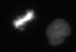
\includegraphics[width=0.25\textwidth]{images/cell_tracking/example_00.png}
                };
                \uncover<2->{
                    \node[transparent_node, red, xshift=-12pt, yshift=5pt] (d11) at (image1.center) {}; 
                    \node[transparent_node, green, xshift=20pt, yshift=-5pt] (d12) at (image1.center) {}; 
                }
            \end{scope}
            \begin{scope}[baseline=(image2.south)]
                \node[right=of image1, xshift=-20pt, label=above:$t+1$] (image2) {
                    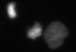
\includegraphics[width=0.25\textwidth]{images/cell_tracking/example_01.png}
                };
                \uncover<3->{
                    \node[transparent_node, red, xshift=-25pt, yshift=15pt] (d21) at (image2.center) {}; 
                    \node[transparent_node, red, xshift=0pt, yshift=-5pt] (d22) at (image2.center) {};
                    \node[transparent_node, green, xshift=18pt, yshift=-10pt] (d23) at (image2.center) {};
                    \path[assignment_arrow, red, bend left=20] (d11) edge (d21);
                    \path[assignment_arrow, red, bend left=10] (d11) edge (d22);
                    \path[assignment_arrow, green, bend right=20] (d12) edge (d23.south west);
                }
            \end{scope}
            \begin{scope}[baseline=(image3.south)]
                \node[right=of image2, xshift=-20pt, label=above:$t+2$] (image3) {
                    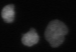
\includegraphics[width=0.25\textwidth]{images/cell_tracking/example_02.png}
                };
                \uncover<4->{
                    \node[transparent_node, red, xshift=-26pt, yshift=13pt] (d31) at (image3.center) {}; 
                    \node[transparent_node, red, xshift=-7pt, yshift=-13pt] (d32) at (image3.center) {};
                    \node[transparent_node, green, xshift=18pt, yshift=-8pt] (d33) at (image3.center) {}; 
                    \path[assignment_arrow, red, bend left=20] (d21) edge (d31);
                    \path[assignment_arrow, red, bend left=20] (d22.north east) edge (d32);
                    \path[assignment_arrow, green, bend right=35] (d23.south east) edge (d33.south west);
                }
            \end{scope}
        \end{tikzpicture}
    \end{figure}
    % \begin{itemize}
    %       \item Extract cell lineages from embryo data.
    %       \item Reconstruct fates of all cells in the embryo.
    %       \item Applicable in 2D and 3D.
    % \end{itemize}
\end{frame}


\begin{frame}
    \frametitle{Struct SVM Tracking Score Function}
    \begin{center}
        \newcommand{\xShift}{100}
        \newcommand{\yShift}{-30}
        \newcommand{\unaryShift}{-17}
        \begin{tikzpicture}[scale=0.5, every node/.append style={transform shape}]

            \node[detection] (d11) {$X_{1}^{1}$};
            \node[detection, below=of d11, yshift=\yShift] (d12) {$X_{2}^{1}$};

            \node[overlay, unaryfac, above=of d11, yshift=\unaryShift, label=left:$\psi_{\text{det}}(X_1^1)$] (u11) {};
            \node[unaryfac, above=of d12, yshift=\unaryShift] (u12) {};

            \path[unaryfac] (d11) -- (u11);
            \path[unaryfac] (d12) -- (u12);


            \foreach \t in {2,...,3}
            {
                \pgfmathtruncatemacro{\currShift}{(\t * 100)}; 
                \pgfmathtruncatemacro{\prevIndex}{(\t - 1)};
                \node[detection, right=of d\prevIndex1, xshift=\xShift] (d\t1) {$X_{1}^{\t}$};
                \node[detection, below=of d\t1, yshift=\yShift] (d\t2) {$X_{2}^{\t}$};
                \node[detection, below=of d\t2, yshift=\yShift] (d\t3) {$X_{3}^{\t}$};

                \node[unaryfac, above=of d\t1, yshift=\unaryShift] (u\t1) {};
                \node[unaryfac, above=of d\t2, yshift=\unaryShift] (u\t2) {};
                \node[unaryfac, above=of d\t3, yshift=\unaryShift] (u\t3) {};

                \path[unaryfac] (d\t1) -- (u\t1);
                \path[unaryfac] (d\t2) -- (u\t2);
                \path[unaryfac] (d\t3) -- (u\t3);
            }

            \foreach \n in {1,...,2}
            {

                \path[transfac] (d1\n) -- (d2\n);
                \path[transfac] (d2\n) -- (d3\n);

                \node[assignment] (y1\n\n) at ($(d2\n)!0.5!(d1\n)$) {$Y_{\n,\n}^{1}$};
                \node[assignment] (y2\n\n) at ($(d2\n)!0.5!(d3\n)$) {$Y_{\n,\n}^{2}$};

                \node[transfac] (out1\n) at ($(d1\n)!0.5!(y1\n\n)$) {};
                \node[transfac] (out2\n) at ($(d2\n)!0.5!(y2\n\n)$) {};
                \node[transfac] (in2\n) at ($(d2\n)!0.5!(y1\n\n)$) {};
                \node[transfac] (in3\n) at ($(d3\n)!0.5!(y2\n\n)$) {};

                
            }

            \node[transfac, label={[yshift=-10]below:$\psi_{\text{in}}(X_3^2, Y_{\bullet,3}^1)$}] (in23) at (in22|-d23) {};
            \node[transfac] (in33) at (in32|-d33) {};
            \node[transfac, label={[yshift=-10]below:$\psi_{\text{out}}(X_3^2, Y_{3,\bullet}^2)$}] (out23) at (out22|-d23) {};

            \path[transfac] (d23) -- (in23);
            \path[transfac] (d23) -- (out23);
            \path[transfac] (d33) -- (in33);

            \path[transfac] (out23) -- (in33);
            \path[transfac] (out12) -- (in21);
            \path[transfac] (out12) -- (in23);
            \path[transfac] (out23) -- (in32);
            \path[transfac] (out22) -- (in31);
            
            \node[assignment] (y233) at ($(d23)!0.5!(d33)$) {$Y_{3,3}^2$};
            \node[assignment] (y121) at ($(d12)!0.5!(d21)$) {$Y_{2,1}^1$};
            \node[assignment] (y123) at ($(d12)!0.5!(d23)$) {$Y_{2,3}^1$};
            \node[assignment] (y232) at ($(d23)!0.5!(d32)$) {$Y_{3,2}^2$};
            \node[assignment] (y221) at ($(d22)!0.5!(d31)$) {$Y_{2,1}^2$};



        \end{tikzpicture}
    \end{center}
    \begin{align}
        \psi_{k} &= \exp(-E_{k}) \\ \nonumber
        E_{k} &= \dualvec{w}_{k}\VEC{\text{features}}_k \\ \nonumber
        F(\text{data}, \text{tracking}; \VEC{w}) &= \sum_k E_k = \dualvec{w}_k\VEC{\text{features}}_k
    \end{align}

\end{frame}



\begin{frame}
    \frametitle{Real Tracking Score}
    \newcommand{\trackingExampleScale}{0.35}
    \begin{center}
        \begin{tikzpicture}
            \node (score) { 
\includegraphics[width=0.85\textwidth]{images/struct_svm_objective_4by3_no-cb.pdf} };
            \begin{scope}[x={($(score.south east)-(score.south west)$)},y={($(score.north
                    west)-(score.south west)$)}, overlay]
                \begin{scope}[axis/.style={very thick, ->, >=stealth'}]
                    \draw[axis] (-0.55, -0.5) -- (0.52, -0.5) node (xaxis) [below] {$w_1$};
                    \draw[axis] (-0.5, -0.55) -- (-0.5, 0.52) node (yaxis) [left]  {$w_2$};
                \end{scope}
                \uncover<1->{ \node[score_tracking] (t0) at ( 0.3, -0.15 ) {\begin{tikzpicture}[scale=\trackingExampleScale, every node/.style={transform shape}]
    \begin{scope}[baseline=(image1.south)]
        \node (image1) {
            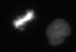
\includegraphics[width=0.25\textwidth]{images/cell_tracking/example_00.png}
        };
        \node[transparent_node, red, xshift=-12pt, yshift=5pt] (d11) at (image1.center) {}; 
        \node[transparent_node, green, xshift=20pt, yshift=-5pt] (d12) at (image1.center) {}; 
    \end{scope}
    \begin{scope}[baseline=(image2.south)]
        \node[right=of image1, xshift=-20pt] (image2) {
            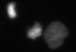
\includegraphics[width=0.25\textwidth]{images/cell_tracking/example_01.png}
        };
        \begin{scope}[overlay]
            \node[transparent_node, red, xshift=-25pt, yshift=15pt] (d21) at (image2.center) {}; 
            \node[transparent_node, red, xshift=0pt, yshift=-5pt] (d22) at (image2.center) {};
            \node[transparent_node, green, xshift=18pt, yshift=-10pt] (d23) at (image2.center) {};
            \path[assignment_arrow, red, bend left=20] (d11) edge (d21);
            \path[assignment_arrow, red, bend left=10] (d11) edge (d22);
            \path[assignment_arrow, green, bend right=20] (d12) edge (d23.south west);
        \end{scope}
    \end{scope}
    \begin{scope}[baseline=(image3.south)]
        \node[right=of image2, xshift=-20pt] (image3) {
            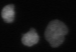
\includegraphics[width=0.25\textwidth]{images/cell_tracking/example_02.png}
        };
        \begin{scope}[overlay]
            \node[transparent_node, red, xshift=-26pt, yshift=13pt] (d31) at (image3.center) {}; 
            \node[transparent_node, red, xshift=-7pt, yshift=-13pt] (d32) at (image3.center) {};
            \node[transparent_node, green, xshift=18pt, yshift=-8pt] (d33) at (image3.center) {}; 
            \path[assignment_arrow, red, bend left=20] (d21) edge (d31);
            \path[assignment_arrow, red, bend left=20] (d22.north east) edge (d32);
            \path[assignment_arrow, green, bend right=35] (d23.south east) edge (d33.south west);
        \end{scope}
    \end{scope}
\end{tikzpicture}


%%% Local Variables: 
%%% mode: latex
%%% TeX-master: "../../../main"
%%% End: 
}; }
                \uncover<2->{ \node[score_tracking] (t1) at ( 0.25, 0.05 ) {\begin{tikzpicture}[scale=\trackingExampleScale, every node/.style={transform shape}]
    \begin{scope}[baseline=(image1.south)]
        \node (image1) {
            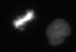
\includegraphics[width=0.25\textwidth]{images/cell_tracking/example_00.png}
        };
        \begin{scope}[overlay]
        \node[transparent_node, red, xshift=-12pt, yshift=5pt] (d11) at (image1.center) {}; 
        \node[transparent_node, green, xshift=20pt, yshift=-5pt] (d12) at (image1.center) {};
        \end{scope}
    \end{scope}
    \begin{scope}[baseline=(image2.south)]
        \node[right=of image1, xshift=-20pt] (image2) {
            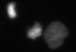
\includegraphics[width=0.25\textwidth]{images/cell_tracking/example_01.png}
        };
        \begin{scope}[overlay]
        \node[transparent_node, red, xshift=-25pt, yshift=15pt] (d21) at (image2.center) {}; 
        \node[transparent_node, red, xshift=0pt, yshift=-5pt] (d22) at (image2.center) {};
        \node[transparent_node, green, xshift=18pt, yshift=-10pt] (d23) at (image2.center) {};
        \path[assignment_arrow, red, bend left=20] (d11) edge (d21);
        \path[assignment_arrow, red, bend left=10] (d11) edge (d22);
        \path[assignment_arrow, green, bend right=20] (d12) edge (d23.south west);
        \end{scope}
    \end{scope}
    \begin{scope}[baseline=(image3.south)]
        \node[right=of image2, xshift=-20pt] (image3) {
            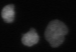
\includegraphics[width=0.25\textwidth]{images/cell_tracking/example_02.png}
        };
        \begin{scope}[overlay]
        \node[transparent_node, red, xshift=-26pt, yshift=13pt] (d31) at (image3.center) {}; 
        \node[transparent_node, red, xshift=-7pt, yshift=-13pt] (d32) at (image3.center) {};
        \path[assignment_arrow, red, bend left=20] (d21) edge (d31);
        \path[assignment_arrow, red, bend left=20] (d22.north east) edge (d32);
        \end{scope}
    \end{scope}
\end{tikzpicture}


%%% Local Variables: 
%%% mode: latex
%%% TeX-master: "../../../main"
%%% End: 
}; }
                \uncover<3->{ \node[score_tracking] (t2) at ( 0.2, 0.4 )  {\begin{tikzpicture}[scale=\trackingExampleScale, every node/.style={transform shape}]
    \begin{scope}[baseline=(image1.south)]
        \node (image1) {
            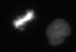
\includegraphics[width=0.25\textwidth]{images/cell_tracking/example_00.png}
        };
    \end{scope}
    \begin{scope}[baseline=(image2.south)]
        \node[right=of image1, xshift=-20pt] (image2) {
            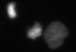
\includegraphics[width=0.25\textwidth]{images/cell_tracking/example_01.png}
        };
    \end{scope}
    \begin{scope}[baseline=(image3.south)]
        \node[right=of image2, xshift=-20pt] (image3) {
            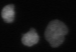
\includegraphics[width=0.25\textwidth]{images/cell_tracking/example_02.png}
        };
    \end{scope}
\end{tikzpicture}


%%% Local Variables: 
%%% mode: latex
%%% TeX-master: "../../../main"
%%% End: 
}; }
                \uncover<4->{ \node[score_tracking] (t3) at ( -0.17, 0.25 ) {\begin{tikzpicture}[scale=\trackingExampleScale, every node/.style={transform shape}]
    \begin{scope}[baseline=(image1.south)]
        \node (image1) {
            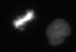
\includegraphics[width=0.25\textwidth]{images/cell_tracking/example_00.png}
        };
        \node[transparent_node, red, xshift=-12pt, yshift=5pt] (d11) at (image1.center) {}; 
        \node[transparent_node, green, xshift=20pt, yshift=-5pt] (d12) at (image1.center) {}; 
    \end{scope}
    \begin{scope}[baseline=(image2.south)]
        \node[right=of image1, xshift=-20pt] (image2) {
            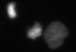
\includegraphics[width=0.25\textwidth]{images/cell_tracking/example_01.png}
        };
        \begin{scope}[overlay]
            \node[transparent_node, red, xshift=-25pt, yshift=15pt] (d21) at (image2.center) {}; 
            \node[transparent_node, green, xshift=0pt, yshift=-5pt] (d22) at (image2.center) {};
            \node[transparent_node, green, xshift=18pt, yshift=-10pt] (d23) at (image2.center) {};
            \path[assignment_arrow, red, bend left=20] (d11) edge (d21);
            \path[assignment_arrow, green, bend left=10] (d12) edge (d22);
            \path[assignment_arrow, green, bend right=20] (d12) edge (d23.south west);
        \end{scope}
    \end{scope}
    \begin{scope}[baseline=(image3.south)]
        \node[right=of image2, xshift=-20pt] (image3) {
            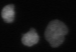
\includegraphics[width=0.25\textwidth]{images/cell_tracking/example_02.png}
        };
        \begin{scope}[overlay]
            \node[transparent_node, red, xshift=-26pt, yshift=13pt] (d31) at (image3.center) {}; 
            \node[transparent_node, green, xshift=-7pt, yshift=-13pt] (d32) at (image3.center) {};
            \node[transparent_node, green, xshift=18pt, yshift=-8pt] (d33) at (image3.center) {}; 
            \path[assignment_arrow, red, bend left=20] (d21) edge (d31);
            \path[assignment_arrow, green, bend left=20] (d22.north east) edge (d32);
            \path[assignment_arrow, green, bend right=35] (d23.south east) edge (d33.south west);
        \end{scope}
    \end{scope}
\end{tikzpicture}


%%% Local Variables: 
%%% mode: latex
%%% TeX-master: "../../../main"
%%% End: 
}; }
                \uncover<5->{ \node[score_tracking] (t4) at ( -0.2, -0.2 ) {\begin{tikzpicture}[scale=\trackingExampleScale, every node/.style={transform shape}]
    \begin{scope}[baseline=(image1.south)]
        \node (image1) {
            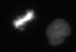
\includegraphics[width=0.25\textwidth]{images/cell_tracking/example_00.png}
        };
        \node[transparent_node, red, xshift=-12pt, yshift=5pt] (d11) at (image1.center) {}; 
        \node[transparent_node, green, xshift=20pt, yshift=-5pt] (d12) at (image1.center) {}; 
    \end{scope}
    \begin{scope}[baseline=(image2.south)]
        \node[right=of image1, xshift=-20pt] (image2) {
            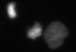
\includegraphics[width=0.25\textwidth]{images/cell_tracking/example_01.png}
        };
        \begin{scope}[overlay]
            \node[transparent_node, red, xshift=-25pt, yshift=15pt] (d21) at (image2.center) {}; 
            \node[transparent_node, green, xshift=18pt, yshift=-10pt] (d23) at (image2.center) {};
            \path[assignment_arrow, red, bend left=20] (d11) edge (d21);
            \path[assignment_arrow, green, bend right=20] (d12) edge (d23.south west);
        \end{scope}
    \end{scope}
    \begin{scope}[baseline=(image3.south)]
        \node[right=of image2, xshift=-20pt] (image3) {
            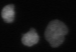
\includegraphics[width=0.25\textwidth]{images/cell_tracking/example_02.png}
        };
        \begin{scope}[overlay]
            \node[transparent_node, red, xshift=-26pt, yshift=13pt] (d31) at (image3.center) {}; 
            \node[transparent_node, green, xshift=18pt, yshift=-8pt] (d33) at (image3.center) {}; 
            \path[assignment_arrow, red, bend left=20] (d21) edge (d31);
            \path[assignment_arrow, green, bend right=35] (d23.south east) edge (d33.south west);
        \end{scope}
    \end{scope}
\end{tikzpicture}


%%% Local Variables: 
%%% mode: latex
%%% TeX-master: "../../../main"
%%% End: 
}; }
                \uncover<6->{
                    \node[font=\small, below=of t0, yshift=31] (w0) {$\textbf{w}^*, b^*$};
                    \node[font=\small, below=of t1, yshift=31] (w1) {$\textbf{w}^{(1)}, b^{(1)}$};
                    \node[font=\small, below=of t2, yshift=31] (w2) {$\textbf{w}^{(2)}, b^{(2)}$};
                    \node[font=\small, below=of t3, yshift=31] (w3) {$\textbf{w}^{(3)}, b^{(3)}$};
                    \node[font=\small, below=of t4, yshift=31] (w4) {$\textbf{w}^{(4)}, b^{(4)}$};
                }
            \end{scope}
        \end{tikzpicture}
    \end{center}

\end{frame}


\begin{frame}
    \frametitle{Tracking Score Obtained From Structured Learning}
    \newcommand{\trackingExampleScale}{0.35}
    \begin{center}
        \begin{tikzpicture}
            \node (score) { 
\includegraphics[width=0.85\textwidth]{images/struct_svm_objective_4by3_no-cb_learned.pdf} };
            \begin{scope}[x={($(score.south east)-(score.south west)$)},y={($(score.north
                    west)-(score.south west)$)}, overlay]
                \begin{scope}[axis/.style={very thick, ->, >=stealth'}]
                    \draw[axis] (-0.55, -0.5) -- (0.52, -0.5) node (xaxis) [below] {$w_1$};
                    \draw[axis] (-0.5, -0.55) -- (-0.5, 0.52) node (yaxis) [left]  {$w_2$};
                \end{scope}
                { \node[score_tracking] (t0) at ( 0.3, -0.15 ) {\begin{tikzpicture}[scale=\trackingExampleScale, every node/.style={transform shape}]
    \begin{scope}[baseline=(image1.south)]
        \node (image1) {
            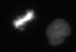
\includegraphics[width=0.25\textwidth]{images/cell_tracking/example_00.png}
        };
        \node[transparent_node, red, xshift=-12pt, yshift=5pt] (d11) at (image1.center) {}; 
        \node[transparent_node, green, xshift=20pt, yshift=-5pt] (d12) at (image1.center) {}; 
    \end{scope}
    \begin{scope}[baseline=(image2.south)]
        \node[right=of image1, xshift=-20pt] (image2) {
            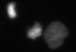
\includegraphics[width=0.25\textwidth]{images/cell_tracking/example_01.png}
        };
        \begin{scope}[overlay]
            \node[transparent_node, red, xshift=-25pt, yshift=15pt] (d21) at (image2.center) {}; 
            \node[transparent_node, red, xshift=0pt, yshift=-5pt] (d22) at (image2.center) {};
            \node[transparent_node, green, xshift=18pt, yshift=-10pt] (d23) at (image2.center) {};
            \path[assignment_arrow, red, bend left=20] (d11) edge (d21);
            \path[assignment_arrow, red, bend left=10] (d11) edge (d22);
            \path[assignment_arrow, green, bend right=20] (d12) edge (d23.south west);
        \end{scope}
    \end{scope}
    \begin{scope}[baseline=(image3.south)]
        \node[right=of image2, xshift=-20pt] (image3) {
            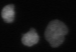
\includegraphics[width=0.25\textwidth]{images/cell_tracking/example_02.png}
        };
        \begin{scope}[overlay]
            \node[transparent_node, red, xshift=-26pt, yshift=13pt] (d31) at (image3.center) {}; 
            \node[transparent_node, red, xshift=-7pt, yshift=-13pt] (d32) at (image3.center) {};
            \node[transparent_node, green, xshift=18pt, yshift=-8pt] (d33) at (image3.center) {}; 
            \path[assignment_arrow, red, bend left=20] (d21) edge (d31);
            \path[assignment_arrow, red, bend left=20] (d22.north east) edge (d32);
            \path[assignment_arrow, green, bend right=35] (d23.south east) edge (d33.south west);
        \end{scope}
    \end{scope}
\end{tikzpicture}


%%% Local Variables: 
%%% mode: latex
%%% TeX-master: "../../../main"
%%% End: 
}; }
                { \node[score_tracking] (t1) at ( 0.25, 0.05 ) {\begin{tikzpicture}[scale=\trackingExampleScale, every node/.style={transform shape}]
    \begin{scope}[baseline=(image1.south)]
        \node (image1) {
            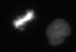
\includegraphics[width=0.25\textwidth]{images/cell_tracking/example_00.png}
        };
        \begin{scope}[overlay]
        \node[transparent_node, red, xshift=-12pt, yshift=5pt] (d11) at (image1.center) {}; 
        \node[transparent_node, green, xshift=20pt, yshift=-5pt] (d12) at (image1.center) {};
        \end{scope}
    \end{scope}
    \begin{scope}[baseline=(image2.south)]
        \node[right=of image1, xshift=-20pt] (image2) {
            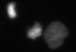
\includegraphics[width=0.25\textwidth]{images/cell_tracking/example_01.png}
        };
        \begin{scope}[overlay]
        \node[transparent_node, red, xshift=-25pt, yshift=15pt] (d21) at (image2.center) {}; 
        \node[transparent_node, red, xshift=0pt, yshift=-5pt] (d22) at (image2.center) {};
        \node[transparent_node, green, xshift=18pt, yshift=-10pt] (d23) at (image2.center) {};
        \path[assignment_arrow, red, bend left=20] (d11) edge (d21);
        \path[assignment_arrow, red, bend left=10] (d11) edge (d22);
        \path[assignment_arrow, green, bend right=20] (d12) edge (d23.south west);
        \end{scope}
    \end{scope}
    \begin{scope}[baseline=(image3.south)]
        \node[right=of image2, xshift=-20pt] (image3) {
            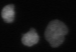
\includegraphics[width=0.25\textwidth]{images/cell_tracking/example_02.png}
        };
        \begin{scope}[overlay]
        \node[transparent_node, red, xshift=-26pt, yshift=13pt] (d31) at (image3.center) {}; 
        \node[transparent_node, red, xshift=-7pt, yshift=-13pt] (d32) at (image3.center) {};
        \path[assignment_arrow, red, bend left=20] (d21) edge (d31);
        \path[assignment_arrow, red, bend left=20] (d22.north east) edge (d32);
        \end{scope}
    \end{scope}
\end{tikzpicture}


%%% Local Variables: 
%%% mode: latex
%%% TeX-master: "../../../main"
%%% End: 
}; }
                { \node[score_tracking] (t2) at ( 0.2, 0.4 )  {\begin{tikzpicture}[scale=\trackingExampleScale, every node/.style={transform shape}]
    \begin{scope}[baseline=(image1.south)]
        \node (image1) {
            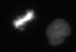
\includegraphics[width=0.25\textwidth]{images/cell_tracking/example_00.png}
        };
    \end{scope}
    \begin{scope}[baseline=(image2.south)]
        \node[right=of image1, xshift=-20pt] (image2) {
            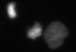
\includegraphics[width=0.25\textwidth]{images/cell_tracking/example_01.png}
        };
    \end{scope}
    \begin{scope}[baseline=(image3.south)]
        \node[right=of image2, xshift=-20pt] (image3) {
            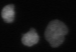
\includegraphics[width=0.25\textwidth]{images/cell_tracking/example_02.png}
        };
    \end{scope}
\end{tikzpicture}


%%% Local Variables: 
%%% mode: latex
%%% TeX-master: "../../../main"
%%% End: 
}; }
                { \node[score_tracking] (t3) at ( -0.17, 0.25 ) {\begin{tikzpicture}[scale=\trackingExampleScale, every node/.style={transform shape}]
    \begin{scope}[baseline=(image1.south)]
        \node (image1) {
            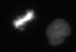
\includegraphics[width=0.25\textwidth]{images/cell_tracking/example_00.png}
        };
        \node[transparent_node, red, xshift=-12pt, yshift=5pt] (d11) at (image1.center) {}; 
        \node[transparent_node, green, xshift=20pt, yshift=-5pt] (d12) at (image1.center) {}; 
    \end{scope}
    \begin{scope}[baseline=(image2.south)]
        \node[right=of image1, xshift=-20pt] (image2) {
            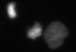
\includegraphics[width=0.25\textwidth]{images/cell_tracking/example_01.png}
        };
        \begin{scope}[overlay]
            \node[transparent_node, red, xshift=-25pt, yshift=15pt] (d21) at (image2.center) {}; 
            \node[transparent_node, green, xshift=0pt, yshift=-5pt] (d22) at (image2.center) {};
            \node[transparent_node, green, xshift=18pt, yshift=-10pt] (d23) at (image2.center) {};
            \path[assignment_arrow, red, bend left=20] (d11) edge (d21);
            \path[assignment_arrow, green, bend left=10] (d12) edge (d22);
            \path[assignment_arrow, green, bend right=20] (d12) edge (d23.south west);
        \end{scope}
    \end{scope}
    \begin{scope}[baseline=(image3.south)]
        \node[right=of image2, xshift=-20pt] (image3) {
            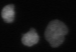
\includegraphics[width=0.25\textwidth]{images/cell_tracking/example_02.png}
        };
        \begin{scope}[overlay]
            \node[transparent_node, red, xshift=-26pt, yshift=13pt] (d31) at (image3.center) {}; 
            \node[transparent_node, green, xshift=-7pt, yshift=-13pt] (d32) at (image3.center) {};
            \node[transparent_node, green, xshift=18pt, yshift=-8pt] (d33) at (image3.center) {}; 
            \path[assignment_arrow, red, bend left=20] (d21) edge (d31);
            \path[assignment_arrow, green, bend left=20] (d22.north east) edge (d32);
            \path[assignment_arrow, green, bend right=35] (d23.south east) edge (d33.south west);
        \end{scope}
    \end{scope}
\end{tikzpicture}


%%% Local Variables: 
%%% mode: latex
%%% TeX-master: "../../../main"
%%% End: 
}; }
                { \node[score_tracking] (t4) at ( -0.2, -0.2 ) {\begin{tikzpicture}[scale=\trackingExampleScale, every node/.style={transform shape}]
    \begin{scope}[baseline=(image1.south)]
        \node (image1) {
            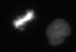
\includegraphics[width=0.25\textwidth]{images/cell_tracking/example_00.png}
        };
        \node[transparent_node, red, xshift=-12pt, yshift=5pt] (d11) at (image1.center) {}; 
        \node[transparent_node, green, xshift=20pt, yshift=-5pt] (d12) at (image1.center) {}; 
    \end{scope}
    \begin{scope}[baseline=(image2.south)]
        \node[right=of image1, xshift=-20pt] (image2) {
            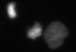
\includegraphics[width=0.25\textwidth]{images/cell_tracking/example_01.png}
        };
        \begin{scope}[overlay]
            \node[transparent_node, red, xshift=-25pt, yshift=15pt] (d21) at (image2.center) {}; 
            \node[transparent_node, green, xshift=18pt, yshift=-10pt] (d23) at (image2.center) {};
            \path[assignment_arrow, red, bend left=20] (d11) edge (d21);
            \path[assignment_arrow, green, bend right=20] (d12) edge (d23.south west);
        \end{scope}
    \end{scope}
    \begin{scope}[baseline=(image3.south)]
        \node[right=of image2, xshift=-20pt] (image3) {
            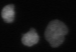
\includegraphics[width=0.25\textwidth]{images/cell_tracking/example_02.png}
        };
        \begin{scope}[overlay]
            \node[transparent_node, red, xshift=-26pt, yshift=13pt] (d31) at (image3.center) {}; 
            \node[transparent_node, green, xshift=18pt, yshift=-8pt] (d33) at (image3.center) {}; 
            \path[assignment_arrow, red, bend left=20] (d21) edge (d31);
            \path[assignment_arrow, green, bend right=35] (d23.south east) edge (d33.south west);
        \end{scope}
    \end{scope}
\end{tikzpicture}


%%% Local Variables: 
%%% mode: latex
%%% TeX-master: "../../../main"
%%% End: 
}; }
                {
                    \node[font=\small, below=of t0, yshift=31] (w0) {$\textbf{w}^*, b^*$};
                    \node[font=\small, below=of t1, yshift=31] (w1) {$\textbf{w}^{(1)}, b^{(1)}$};
                    \node[font=\small, below=of t2, yshift=31] (w2) {$\textbf{w}^{(2)}, b^{(2)}$};
                    \node[font=\small, below=of t3, yshift=31] (w3) {$\textbf{w}^{(3)}, b^{(3)}$};
                    \node[font=\small, below=of t4, yshift=31] (w4) {$\textbf{w}^{(4)}, b^{(4)}$};
                }
            \end{scope}
        \end{tikzpicture}
    \end{center}

\end{frame}




\begin{frame}
    \frametitle{Struct SVM Tracking Score Function Augmented By Hamming Loss}
    \begin{center}
        \newcommand{\xShift}{100}
        \newcommand{\yShift}{-30}
        \newcommand{\unaryXShift}{22}
        \newcommand{\unaryShift}{-\unaryXShift}
        \begin{tikzpicture}[scale=0.5, every node/.append style={transform shape}]

            \node[detection] (d11) {$X_{1}^{1}$};
            \node[detection, below=of d11, yshift=\yShift] (d12) {$X_{2}^{1}$};

            \node[overlay, unaryfac, above left=of d11, yshift=\unaryShift, xshift=\unaryXShift, label=left:$\psi_{\text{det}}(X_1^1)$] (u11) {};
            \node[unaryfac, above left=of d12, yshift=\unaryShift, xshift=\unaryXShift] (u12) {};

            \path[unaryfac] (d11) -- (u11);
            \path[unaryfac] (d12) -- (u12);

            \node[lossfac, above right=of d11, yshift=\unaryShift, xshift=-\unaryXShift, label=right:loss] (l11) {};
            \node[lossfac, above right=of d12, yshift=\unaryShift, xshift=-\unaryXShift] (l12) {};

            \path[lossfac] (d11) -- (l11);
            \path[lossfac] (d12) -- (l12);


            \foreach \t in {2,...,3}
            {
                \pgfmathtruncatemacro{\currShift}{(\t * 100)}; 
                \pgfmathtruncatemacro{\prevIndex}{(\t - 1)};
                \node[detection, right=of d\prevIndex1, xshift=\xShift] (d\t1) {$X_{1}^{\t}$};
                \node[detection, below=of d\t1, yshift=\yShift] (d\t2) {$X_{2}^{\t}$};
                \node[detection, below=of d\t2, yshift=\yShift] (d\t3) {$X_{3}^{\t}$};

                \node[unaryfac, above left=of d\t1, yshift=\unaryShift, xshift=\unaryXShift] (u\t1) {};
                \node[unaryfac, above left=of d\t2, yshift=\unaryShift, xshift=\unaryXShift] (u\t2) {};
                \node[unaryfac, above left=of d\t3, yshift=\unaryShift, xshift=\unaryXShift] (u\t3) {};

                \node[lossfac, above right=of d\t1, yshift=\unaryShift, xshift=-\unaryXShift] (l\t1) {};
                \node[lossfac, above right=of d\t2, yshift=\unaryShift, xshift=-\unaryXShift] (l\t2) {};
                \node[lossfac, above right=of d\t3, yshift=\unaryShift, xshift=-\unaryXShift] (l\t3) {};

                \path[unaryfac] (d\t1) -- (u\t1);
                \path[unaryfac] (d\t2) -- (u\t2);
                \path[unaryfac] (d\t3) -- (u\t3);

                \path[lossfac] (d\t1) -- (l\t1);
                \path[lossfac] (d\t2) -- (l\t2);
                \path[lossfac] (d\t3) -- (l\t3);
            }

            \foreach \n in {1,...,2}
            {

                \path[transfac] (d1\n) -- (d2\n);
                \path[transfac] (d2\n) -- (d3\n);

                \node[assignment] (y1\n\n) at ($(d2\n)!0.5!(d1\n)$) {$Y_{\n,\n}^{1}$};
                \node[assignment] (y2\n\n) at ($(d2\n)!0.5!(d3\n)$) {$Y_{\n,\n}^{2}$};

                \node[transfac] (out1\n) at ($(d1\n)!0.5!(y1\n\n)$) {};
                \node[transfac] (out2\n) at ($(d2\n)!0.5!(y2\n\n)$) {};
                \node[transfac] (in2\n) at ($(d2\n)!0.5!(y1\n\n)$) {};
                \node[transfac] (in3\n) at ($(d3\n)!0.5!(y2\n\n)$) {};

                \node[lossfac, above right=of y1\n\n, yshift=\unaryShift, xshift=-\unaryXShift]
                (l1\n\n) {};
                \node[lossfac, above right=of y2\n\n, yshift=\unaryShift, xshift=-\unaryXShift]
                (l2\n\n) {};

                \path[lossfac] (y1\n\n) -- (l1\n\n);
                \path[lossfac] (y2\n\n) -- (l2\n\n);
                
            }

            \node[transfac, label={[yshift=-10]below:$\psi_{\text{in}}(X_3^2, Y_{\bullet,3}^1)$}] (in23) at (in22|-d23) {};
            \node[transfac] (in33) at (in32|-d33) {};
            \node[transfac, label={[yshift=-10]below:$\psi_{\text{out}}(X_3^2, Y_{3,\bullet}^2)$}] (out23) at (out22|-d23) {};

            \path[transfac] (d23) -- (in23);
            \path[transfac] (d23) -- (out23);
            \path[transfac] (d33) -- (in33);

            \path[transfac] (out23) -- (in33);
            \path[transfac] (out12) -- (in21);
            \path[transfac] (out12) -- (in23);
            \path[transfac] (out23) -- (in32);
            \path[transfac] (out22) -- (in31);
            
            \node[assignment] (y233) at ($(d23)!0.5!(d33)$) {$Y_{3,3}^2$};
            \node[assignment] (y121) at ($(d12)!0.5!(d21)$) {$Y_{2,1}^1$};
            \node[assignment] (y123) at ($(d12)!0.5!(d23)$) {$Y_{2,3}^1$};
            \node[assignment] (y232) at ($(d23)!0.5!(d32)$) {$Y_{3,2}^2$};
            \node[assignment] (y221) at ($(d22)!0.5!(d31)$) {$Y_{2,1}^2$};



        \end{tikzpicture}
    \end{center}
    \begin{align}
        \psi_{k} &= \exp(-E_{k}) \\ \nonumber
        E_{k} &= \dualvec{w}_{k}\VEC{\text{features}}_k \\ \nonumber
        F(\text{data}, \text{tracking}; \VEC{w}) &= \sum_k E_k = \dualvec{w}_k\VEC{\text{features}}_k
    \end{align}

\end{frame}






    %%% Local Variables: 
    %%% mode: latex
    %%% TeX-master: "../main"
    %%% End: 
